\documentclass{cmspaper}
\usepackage{lineno}
\linenumbers
\usepackage{feynmf}	
\usepackage{graphics}
\usepackage{graphicx}
\usepackage{amssymb,epsfig}
\usepackage{epstopdf}
\usepackage{verbatim}
\usepackage{amsmath}    % need for subequations
\usepackage{draftcopy}
\usepackage{enumerate}
\usepackage{lscape}
\usepackage{sidecap}

%\usepackage{feynmp}
\usepackage{commath}
\usepackage{setspace}
\usepackage{epsfig}
\usepackage{hyperref}
%%%%%%%%%%%%%%%%%%%%%%%%%%%%%%%%%%%%%%%%%%%%%%%%%%%%%%%%%%%%%%%%%%%%%%%%%%%%%%%%%%%%%%%%%%%%%%%%%%%%%%%%%%%%%%%%%%%%%%%%%
%\usepackage{datetime}
%\usepackage{caption}


\begin{document}
%==============================================================================
% title page for few authors
%%%%%%%%%%%%%%%%%%%%--------the lines are commented used %% for iCMS analysis note----------%%%%%%%%%%%%%%
%%\begin{titlepage}

% select one of the following and type in the proper number:
%  \cmsnote{2005/000}
%%  \internalnote{}
%  \conferencereport{2005/000}

%%\date{\today}
%%\title{Search for a Heavy Higgs in $H \rightarrow t\overline{t}$ channel at 13 TeV using CMS data}
%%\begin{Authlist}
%%Muhammad Gul, Bugra Bilin, Efe Yazgan, Michael Tytgat
%%Ghent University, Belgium \\
%%METU, Ankara, Turkey
%%\end{Authlist}

% if needed, use the following:
%\collaboration{Flying Saucers Investigation Group}
%\collaboration{CMS collaboration}
% \Anotfoot{a}{On leave from prison}
%\Anotfoot{b}{Now at the Moon}

%%\begin{abstract}

%%\end{abstract} 

% if needed, use the following:
%\conference{Presented at {\it Physics Rumours}, Coconut Island, April 1, 2005}
%\submitted{Submitted to {\it Physics Rumours}}

%%\note{We search for a heavy higgs boson with a mass upto 1 TeV using CMS proton-proton data at $\sqrt{13}$ TeV. $H \rightarrow t\overline{t}$ channel is used where $t\overline{t}$ decays semileptonically. This channel is clouded by a large irreducible SM $t\overline{t}$ background. The signal $gg \rightarrow H \rightarrow t\overline{t}$ and background $gg \rightarrow t\overline{t}$ interfere, resulting in a peak-dip structure around the heavy Higgs mass values.}
  
%%\end{titlepage}

\tableofcontents

\newpage
\clearpage

\setcounter{page}{2}

\section{Introduction}
The discovery of the Higgs boson by CMS \cite{HiggsCMS} and ATLAS \cite{HiggsATLAS} in July 2012 was not only the confirmation of the Higgs sector in the Standard Model, but also many consequencies on BSM. These results strongly support the Higgs mechanism of electroweak symmetry breaking, but don't exclude the possibility of any additional Higgs state with mass range below or around 1 TeV. A number of searches are devoted to additional spin-zero particles at the LHC, but until now all of them are negative \cite{5584}. There are many extensions of the SM, like MSSM, 2HDM \cite{2HDM}. In the Standard Model the simplest possible scalar structure is assumed ( one SU(2) doublet ) that has only one Higgs boson; on the contrary, its extensions like 2HDM produces a spectrum of physical particles which consists of five spin 0 particles, two of them are chareged H$^\pm$, two are neutral H$^\circ$, h$^\circ$ and one is pseudo-scalar A$^\circ$. \\
Different types of possibilities must be take into account to search these particles. One possibility is to reduce the couplings of one of these Higgs particle to the weak vector bosons - or even zero as in the case of pseudo-scalar - where its couplings to fermions enhanced with respect to the SM Higgs couplings \cite{SignHiggs}. The Higgs sector in the above mentioned models have strong Youkawa couplings to the top quark in the small vacuum expectation value. Hence decay of neutral H$^\circ$ to $t\overline{t}$ becomes dominant. At tree level the pseudo-scalar A$^\circ$ particle can't decay into WW and ZZ and the only mode of decay is $t\overline{t}$. This makes the pseudo-scalar A$^\circ$ more interesting.\\
This analysis presents the search of a Higgs boson, with zero or supressed couplings to the weak vector bosons, via the $t\overline{t}$ channel. The signal $gg\rightarrow H\rightarrow t\overline{t}$ and backgound $gg\rightarrow t\overline{t}$ interfere, which results into a peak-dip structure at the Higgs mass. This phenomenon is clear from generator level and reconstructed level.\\
%----------------------------------------------------------------------------------------------------
\section{CMS Detector}
CMS is a general purpose detector with distinguished feature of superconducting solenoid of 6m internal diameter, providing a magnetic field of 3.8 T \cite{magnet}. The bore of superconducting coil is enough large to accommodate the silicon pixel and strip tracker, a lead tungstate crystal electromagnetic calorimeter (ECAL) and a brass and scintillator hadron callorimeter (HCAL), each of them have a barrel and endcap sections. The return field is large enough to saturate 1.5 m of iron yoke outside the solenoid. Gas-ionizing detectors are installed in 4 stations in the iron yoke for muon detection. Each muon station consists of several layers of aluminium Drift Tubes (DT) in the barrel region and Cathode Strip Chambers (CSC) in the endcap region, complemented by Resistive Plate Chambers (RPC) \cite{rpc}.\\
Two beams of protons from opposite side make a collision at the center of CMS and the resultant particles dump their energy at different parts of the detector. CMS uses paricle-flow (PF) reconstructed algorithm for reconstruction and identification of each individual particle from different parts of the detector. The energy of photon is directly measured from the ECAL. The electron energy is obtained from a combination of the electron momentum determined by the tracker, the energy of the corresponding ECAL cluster and the energy sum of all bremsstrahlung photons originating from the electron track. The energy of muon is measured from the curvature of track in tracker and muon detectors. The energy of charged hadrons is determined from a combination of their momentum measured in the tracker and the matching ECAL and HCAL energy deposits, corrected for zero-suppression effects and for the response function of the calorimeters to hadronic showers. The energy of neutral hadrons is obtained from the corresponding corrected ECAL and HCAL energy.   
More information about the CMS detector, its coordinate system and the relevant kinematic variables can be found in Ref \cite{cmsdetector}. 
%----------------------------------------------------------------------------------------------------
\section{Signal MC Generation and Simulation} 
In this analysis we are searching for a spin-0 particle (scalar and pseudo-scalar) with $m_{H/A} > m_{t\overline{t}}$ in the topBSM. The signal MC is generated using MadGraph \cite{madgraph} generator with the implementation of new physics in the top pair production. A spin-0 particle is added to the SM, with coupling strength to the top quark,
\begin{equation}\label{signalEqu}
g_{S_{0}t\overline{t}} = a_{1}\frac{m_{t}}{v}i + a_{2}\frac{m_{t}}{v}\gamma_{5};
\end{equation} 
is proportional to the top quark mass. Due to large mass of top quark, the coupling is $\approx 1$. In analogy with the SM, $v$ is the spin-0 field vacuum expectation value, $a_{1}$ is the real proportionality constant to the scalar coupling and $a_{2}$ is to the pseudo-scalar coupling. The width of scalar and pseudo-scalar is given by \ref{higgswidth}; 
\begin{equation}\label{higgswidth}
\Gamma_{H} = \frac{3a_{1}m_{t}^{2}m_{H}}{8\pi v^{2}}\beta^{3} \qquad\& \qquad \Gamma_{A} = \frac{3a_{2}m_{t}^{2}m_{A}}{8\pi v^{2}}\beta
\end{equation}
where $\beta = \sqrt{1-\frac{4m_{t}^{2}}{\hat{S}}}$ and $\hat{S} = m_{t\overline{t}}^{2}$.\\
The quark anti-quark annihilation $( q\overline{q}\rightarrow H/A )$ is neglected, because of its large cross section compared to the loop induced gluon fusion process and small branching ratio for scalar to $t\overline{t}$ \cite{signal1}.
Since we are interested in spin-0 bosons with strong couplings to top quark, we neglect all particles in the loop of Fig. \ref{feynSig}(a) except the top quark. We consider a spin-0 particle decaying into ttbar pair, its mass have to be greater than twice the mass of the top quark. The loop induced by gluon-gluon-(pseudo)scalar coupling develops an imaginary part. This leads to a peak-dip structure for interference terms between signal $( gg \rightarrow H/A \rightarrow t\overline{t} )$ and SM background $( gg \rightarrow t\overline{t} )$ just above the mass of spin-0 particle \cite{signal2}, \cite{signal3}.  This behavior is shown in the Fig. \ref{genPlots}.\\
To produce signal MC with interference effect, we have to produce spin-0 particle from gluon fusion decaying into $t\overline{t} ( gg \rightarrow H/A \rightarrow t\overline{t} )$ and the SM production of $t\overline{t}$ from the gluon fusion $( gg \rightarrow t\overline{t} )$ at the same time. MadGraph gives the opportunity to compute the matrix element for the full process $gg \rightarrow t\overline{t}$, which includes the SM and BSM production of ttbar. The Feynman diagrams for those process are given in Fig. \ref{feynSig}. We changed the matrix element by hand and removed all the matrix elements that don’t contribute to the signal. The square of the matrix element for signal as well as the interference terms of the signal $( gg \rightarrow H/A \rightarrow t\overline{t} )$ and background $( gg \rightarrow t\overline{t} )$ are kept. For more technical detail see \cite{signal4}. The full matrix element is given by \ref{matEqu}:
\begin{equation}\label{matEqu}
\mathcal{M}^{2} \propto \mathcal{M}^{2}_{a} + \mathcal{M}_{a}\mathcal{M}^{*}_{c} + \mathcal{M}_{a}\mathcal{M}^{*}_{d} + c.c
\end{equation}
The Equ. \ref{matEqu} shows the interference between diagrams (a) and (d) and diagrams (a) and (c) while diagram (b) doesn’t interfere with (a) because both are s-channels. The output of this method consists of both positive and negative weights correspond to the signal $( gg \rightarrow H/A \rightarrow t\overline{t} )$ and background $( gg \rightarrow t\overline{t} )$. The combination of both gives the interference, produce a peak-dip structure shown in Fig. {genPlots}. This study has already done at $\sqrt{s} = 8$ TeV \cite{sabisteinPAS}.\\
We produced two types of signal MC, one for scalar with $a_{1}$ = 1 and $a_{2}$ = 0 and another for seudo-scalar with $a_{1}$ = 0 and $a_{2}$ = 1 \ref{signalEqu}. The mass ranges are considered from 400 GeV up to 1.2 TeV with a step of 100 GeV for both types of spin-0 particles. Fig. [\ref{xsec_mass}] shows plot of mass versus cross section for both scalar and pseudo scalar particles. Two million events are produced for each sample.\\
For Simulation we used FastSim 2015 recipe\cite{fastsim}, a package available in the CMSSW framework which takes into account generation, simulation, reconstruction and HLT steps. This gives AODSIM format which converted further into MINIAOD format. 
%----------------------------------
\begin{figure}[htp]
\centering
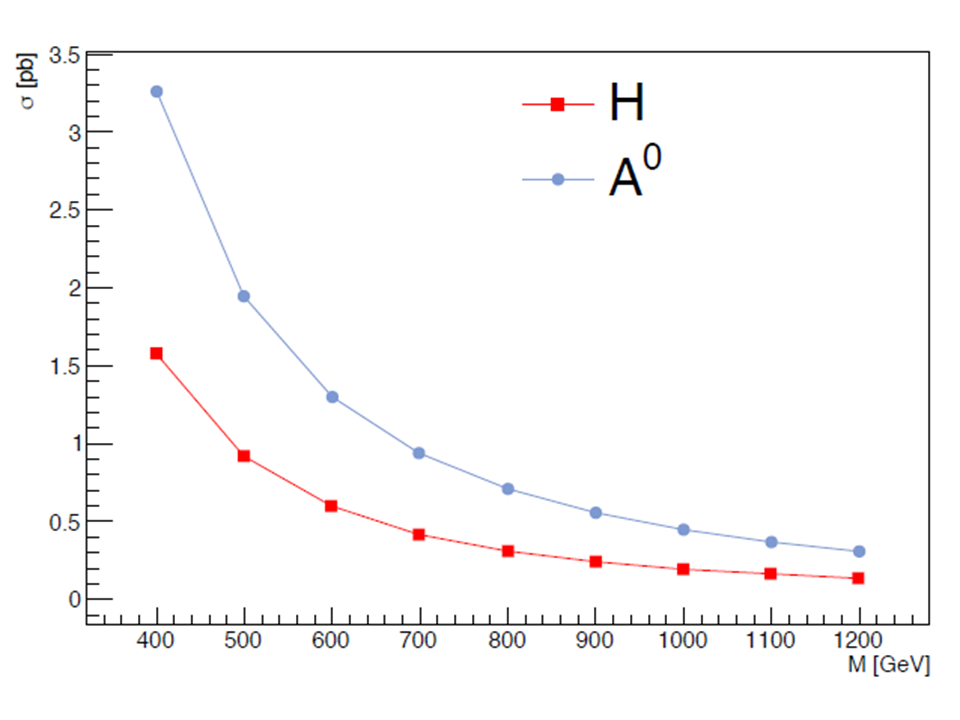
\includegraphics[scale=0.50]{diagrams/xsec_mass.png}
\caption{Cross section versus mass plot for scalar and pseudo scalar particles.}\label{xsec_mass}
\end{figure}
%----------------------------------
\begin{figure}[htp]
\centering
\begin{tabular}{cc}
\hspace{-0.5cm}

\includegraphics[scale=0.53]{diagrams/signal.png}
& \hspace{0.2cm} 
\includegraphics[scale=0.50]{diagrams/SMsignal_b.png}\\
   $(\mathbf{a}): gg\rightarrow H/A \rightarrow t\overline{t}$\qquad\qquad&$(\mathbf{b}): gg \rightarrow t\overline{t}$\\ \\
\hspace{-0.5cm}

\includegraphics[scale=0.50]{diagrams/SMsignal_c.png}
& \hspace{0.2cm} 
\includegraphics[scale=0.50]{diagrams/SMsignal_d.png}\\
   $(\mathbf{c}): gg \rightarrow t\overline{t}$\qquad\qquad&$(\mathbf{d}): gg \rightarrow t\overline{t}$\\
\end{tabular}
\caption{Feynman diagrams for $t\overline{t}$ production. (a): Beyond the Standard Model. (b), (c), (d): The Standard Model.}\label{feynSig}
\end{figure}

  
\begin{figure}[htp]
\centering
\begin{tabular}{cc}
\hspace{-0.5cm}
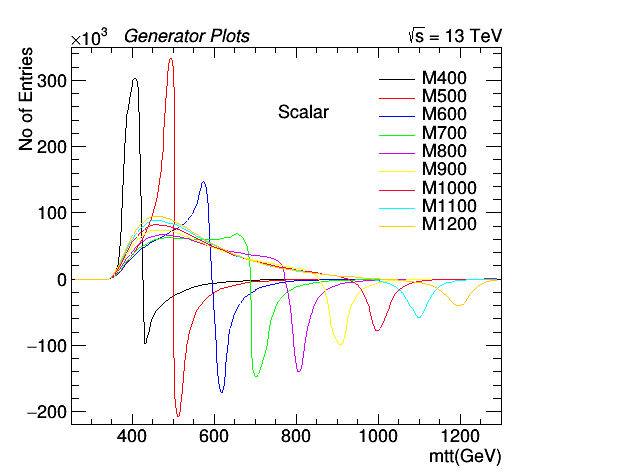
\includegraphics[scale=0.42]{genPlots/mtt_scalar.png}
& \hspace{-1.2cm} 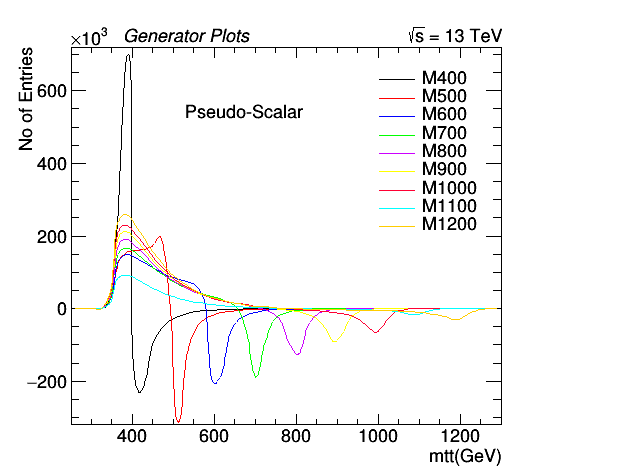
\includegraphics[scale=0.42]{genPlots/mtt_pscalar.png}\\
   ($\mathbf{a}$)\qquad\qquad&($\mathbf{b}$)\qquad\qquad\qquad\\
\hspace{-0.5cm}
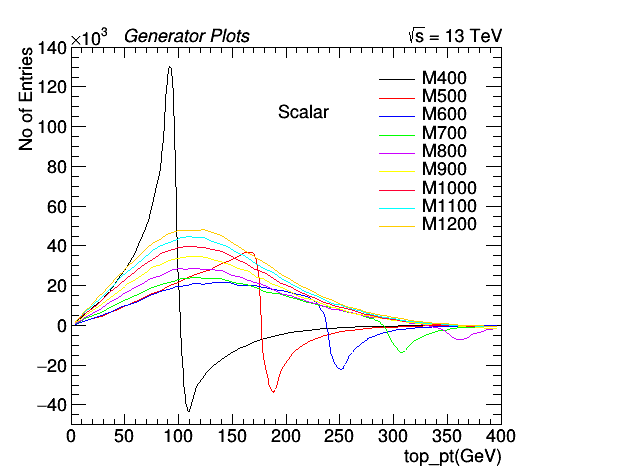
\includegraphics[scale=0.42]{genPlots/top_pt_scalar.png}
& \hspace{-1.2cm} 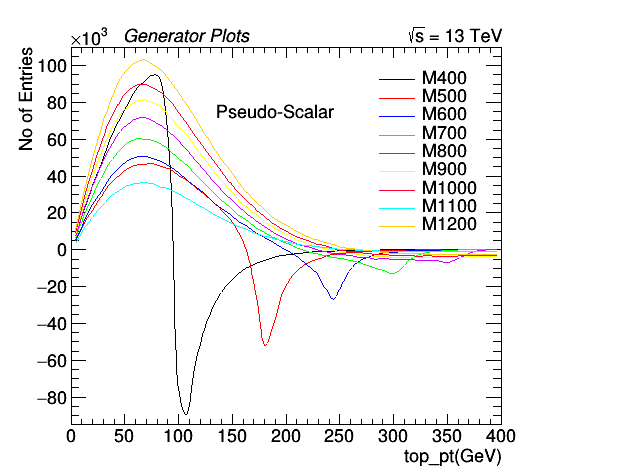
\includegraphics[scale=0.42]{genPlots/top_pt_pscalar.png}\\
   ($\mathbf{c}$)\qquad\qquad&($\mathbf{d}$)\qquad\qquad\qquad\\
\end{tabular}
\caption{Generator level plots with interference effect. (a): Mass of $t\overline{t}$ (scalar) (b): Mass of $t\overline{t}$ (pseudo-scalar) (c): $p_{T}$ of top (scalar) (d): $p_{T}$ of top (pseudo-scalar)}.\label{genPlots}
\end{figure}

%--------------------------------------------------------  
\section{Data and Monte Carlo Samples}
The data set paths with JSON file are given in table [\ref{data_path}] while Monte Carlo (MC) samples used for this analysis are given in table~[\ref{MC-samples}].\\
For simplicity we use [*] = RunIISpring15DR74-Asympt25ns\_MCRUN2\_74\_
%--------------------------
\begin{table*}[h]
     \centering
      \begin{tabular}{rrr}
       \hline
        Name & Path & $\mathcal{L} (fb^{-1}$) \\
\hline
2015D & /SingleMuon/Run2015D-PromptReco-v3 & 0.552 \\
2015D & /SingleMuon/Run2015D-PromptReco-v4 & 1.54 \\
JSON & Cert\_246908-260627\_13TeV\_PromptReco\_Collisions15\_25ns\_JSON.txt & 2.11 \\
\hline
     \end{tabular}
     \caption{Data 2015D with corresponding luminosity.}
     \label{data_path}
\end{table*}
%--------------------------

\begin{table*}[h]
     \begin{tabular}{rrr}
       \hline
         Path & $\sigma$ (pb) & Events \\
\hline
/TT\_TuneCUETP8M1\_13TeV-powheg-pythia8/[*]V9-v2&831.76&19799590 \\
/WJetsToLNu\_TuneCUETP8M1\_13TeV-amcatnloFXFX-pythia8/[*]V9-v1 & 61526.7 & 24151270 \\
/QCD\_Pt-20toInf\_MuEnrichedPt15\_TuneCUETP8M1\_13TeV\_pythia8-/[*]V9A-v2 & 10.43 & 1981954 \\
/ST\_tW\_top\_5f\_inclusiveDecays\_13TeV-powheg-pythia8\_TuneCUETP8M1/[*]V9-v1  & 35.6 & 995600 \\
/ST\_s-channel\_4f\_leptonDecays\_13TeV-amcatnlo-pythia8\_TuneCUETP8M1/[*]V9-v1 & 11.36 & 984400 \\
/ST\_t-channel\_top\_4f\_leptonDecays\_13TeV-powheg-pythia8\_TuneCUETP8M1/[*]V9-v1&43.798 & 3299800 \\
/ST\_tW\_antitop\_5f\_inclusiveDecays\_13TeV-powheg-pythia8\_TuneCUETP8M1/[*]V9-v1  & 1.44 & 95.819 \\
/ST\_t-channel\_antitop\_4f\_leptonDecays\_13TeV-powheg-pythia8\_TuneCUETP8M1/[*]V9-v1  & 26.0659 & 1695400 \\

 \hline
    \end{tabular}
     \caption{Monte Carlo samples with cross sections, number of events and the perturbative order of calculations.}
     \label{MC-samples}
\end{table*}
%-----------------------------------
\section{Event Reconstruction and Selection}
\subsection{Event Selection}
This analysis considers mass of $t\overline{t}$ $\sim$ 1 TeV in semileptonic state. Lepton is either electron or muon. The final state of $t\overline{t}$ is recognized by the decay products of the two W bosons and the two b-jets that they yield. This type of events have one isolated lepton (electron/muon), $\not\mathrel{E}_{T}$ and four jets (two of them are b tagged). Lepton and jets are isolated by a cone with $\triangle R = \sqrt{(\triangle \phi)^2 + (\triangle \eta)^2} >$ 0.4.\\
The number of lepton is selected to be exactly one with $p_{T} > 20$ GeV and $\abs {\eta} < 2.1$. This selection supresses the full leptonic decay of $t\overline{t}$, and the Drell-Yan. The number of jets is at least four, two of them are b jets. This minimizes the hadronic decay of $t\overline{t}$ that consists of six jets and the QCD backgounds. Combined Inclusive Secondary Vertex (CSVv2) is applied for b-tag jets.
%--------------------------------------------------
\subsection{Muon Identification \& Isolation}
The the semileptonic channel of $t\overline{t}$ requires only one lepton. We consider lepton to be muon coming from the decay of W boson. To reconstruct W boson from $\mu$ and $\not\mathrel{E}_{T}$, we need a high efficiency and well isolated muon. Muon is selected using the following identification (ID) criteria \cite{muonid}.
\begin{itemize}
\item muon identified as PFMuon \& Global muon;
\item at least one muon chamber hit included in the global-muon track fit;
\item muon segments in at least two muon stations, to obtain a meaningful estimate of muon $p_{T}$;
\item tracker track transverse impact parameter $d_{xy} <$ 2 mm w.r.t. the primary vertex. It supresses cosmic muons and further supresses muons from decay in flight;
\item longitudinal impact parameter $d_{z} <$ 5 mm;
\item number of pixel hits $>$ 0;
\item number of tracker layers with hits larger than five.
\end{itemize}
On the top of the above selection, relative isolation with $\beta$ correction has applied. 
\begin{equation}
I^{\mu}_{rel} = \frac{(I_{CH} + max(I_{pho}+I_{NH} - 0.5*I_{CH}^{PU},0.))}{P^{\mu}_{T}}
\end{equation}
\subsection{Jets Identification}
This analysis uses ``slimmedJets" that are particle-flow (PF) jets and clustered using anti-kt jet clustering algorithm \cite{Akt}\cite{jet-reco}. Jet energy corrections (JEC) applied (L1FastJet, L2Relative, L3Absolute and L2L3Residual). Jets are selected with $p_{T} > 30$ GeV and $\abs {\eta} < 2.4$ that passes the loose jet Id criterian.
\begin{itemize}
\item Number of constituents $>$ 1
\item Neutral hadron energy fraction $<$ 0.99
\item Neutral electromagnetic fraction $<$ 0.99
\item If $\abs {\eta} < 2.4$, charge multiplicity $>$ 0.0 
\item If $\abs {\eta} < 2.4$, charge hadron energy fraction $>$ 0.0
\item If $\abs {\eta} < 2.4$, Charge electromagnetic fraction $<$ 0.99
\end{itemize}   
\subsubsection{B-tagging}
The identification of b-jet is very important for the study of top quark decays, Higgs decay and many new physics phenomena \cite{bjet}. b tagging is a reconstruction technique that takes advantage of the b hadron properties and assigns to each jet a likelihood that contains a b hadron. Following are the b-jets characteristics which discreminate them from jets produced by light quarks and gluons.
\begin{itemize}
\item Long life time: $\tau \sim$ 1.5 ps, $c\tau \sim$ 450 $\mu $m
\item Large mass: mass $\sim$ 4.2 GeV 
\item High track multiplicity $\sim$ 4-5
\item Large semileptonic branching fraction 
\end{itemize}
We use the Combined Secondary Vertex version 2 (CSVv2) algorithm, based on secondary vertex and track-based lifetime information. It is an updated version of the CSV algorithm used in Run I. CSVv2 combines the variables with a neural network and secondary vertex information is obtained with the Inclusive Vertex Finder algorithm. Three operating points are defined for CSVv2.
Loose (CSVv2L), medium (CSVv2M) and Tight operating points (CSVv2T); for which the rate of misidentifying a light jet as a bjet is 10\%, 1\% and 0.1\% respectively.
CSVv2 has higher effeciency and low mistag rate as compare to other btagging algorithms. This behaviour can be seen using the performance plots for different types of b-tagging algorithms as shown in the Fig.~[\ref{performance_CSVv2}]. Such performance plots usually contains several performance curves typically defined as the mistag rate as a function of the b-tagging efficiency. From the plots it is clear that CSVv2 has higher efficiency and low mistag as compare to other b-tagging algorithms.   

%----------------------------------------------------------------------------------------------------
\begin{figure}[htp]
\centering
\begin{tabular}{cc}
\hspace{-0.5cm}
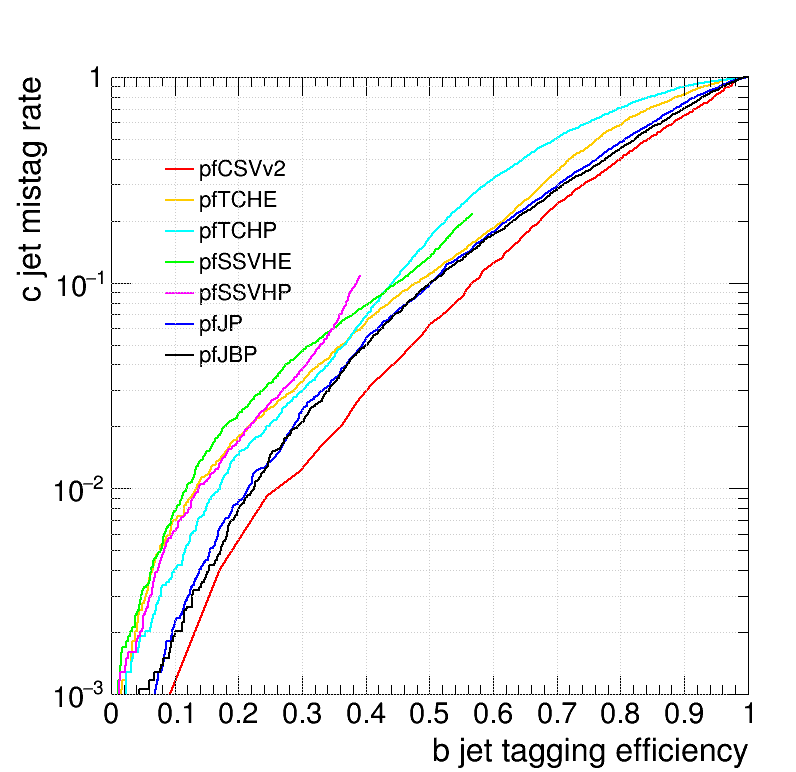
\includegraphics[scale=0.30]{genPlots/btagged/bTagEffVsMistagRate_c.png}
& \hspace{-0.60cm} 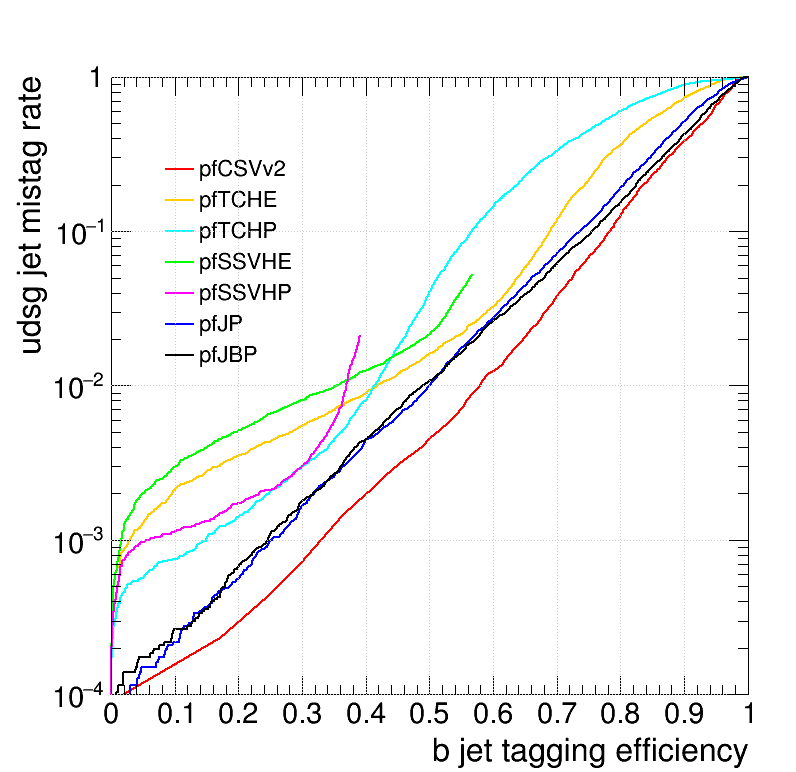
\includegraphics[scale=0.30]{genPlots/btagged/bTagEffVsMistagRate_udsg.png}\\
   ($\mathbf{a}$)\qquad\qquad&($\mathbf{b}$)\qquad\qquad\qquad\\
\end{tabular}
\caption{Log view of the performance plots of CSVv2 (a): b jets tagging efficincy versus c jets mistag rate (b): b jets tagging efficincy versus udsg jets mistag rate}.\label{performance_CSVv2}
\end{figure}
%----------------------------------------------------------------------------------------------------
\begin{figure}[htp]
\centering
\begin{tabular}{cc}
\hspace{-0.5cm}
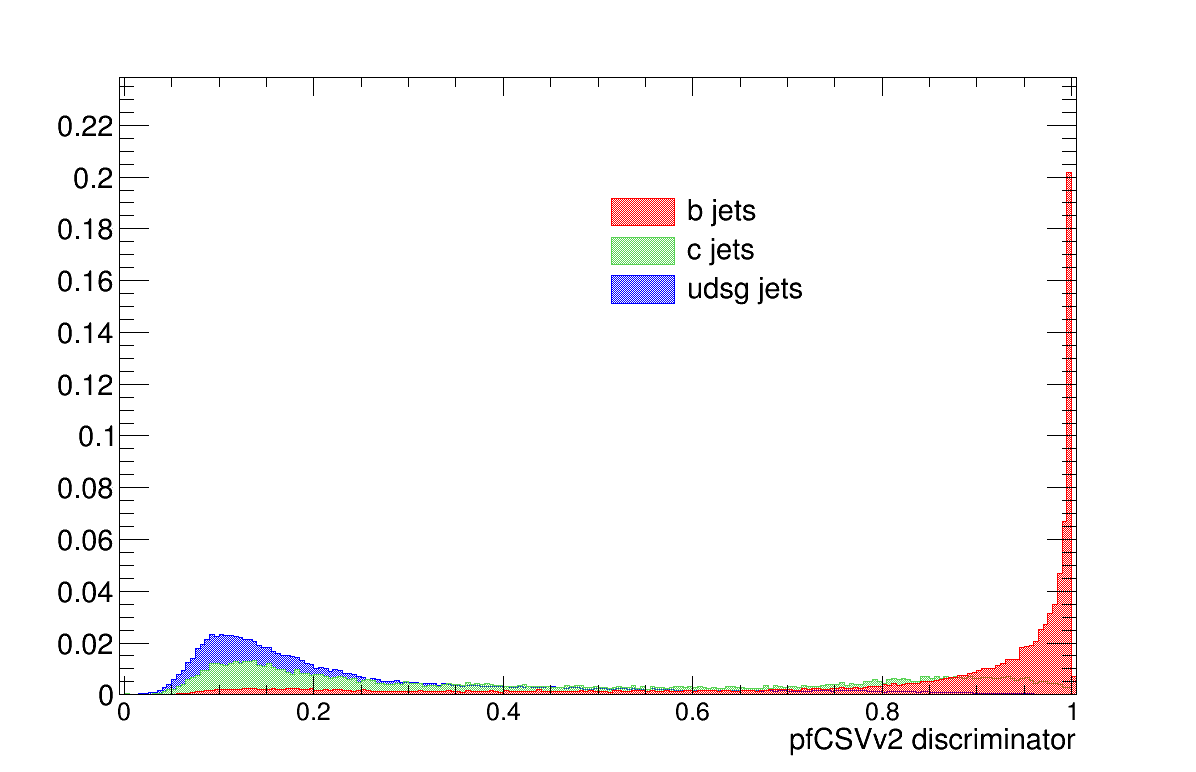
\includegraphics[scale=0.20]{genPlots/btagged/pfCSVv2IVF_discriminator.png}
& \hspace{-0.5cm} 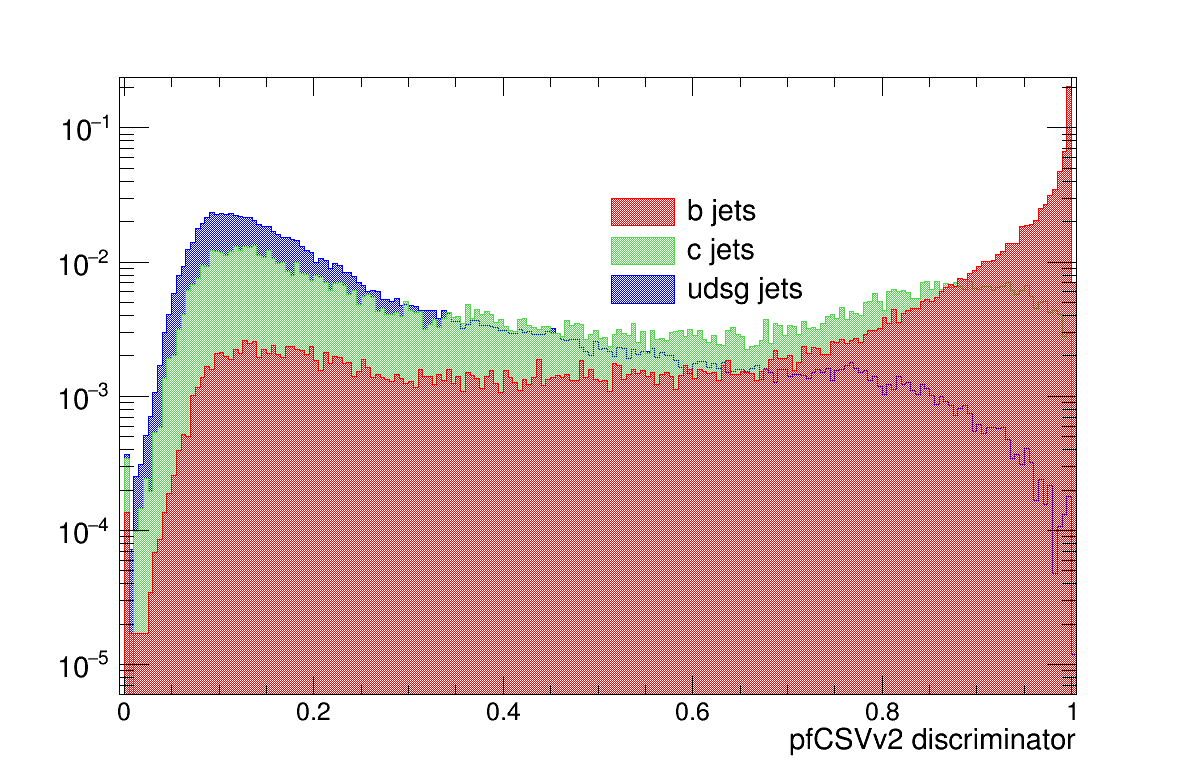
\includegraphics[scale=0.20]{genPlots/btagged/pfCSVv2IVF_discriminator_log.png}\\
   ($\mathbf{a}$)\qquad\qquad&($\mathbf{b}$)\qquad\qquad\qquad\\
\hspace{-0.5cm}
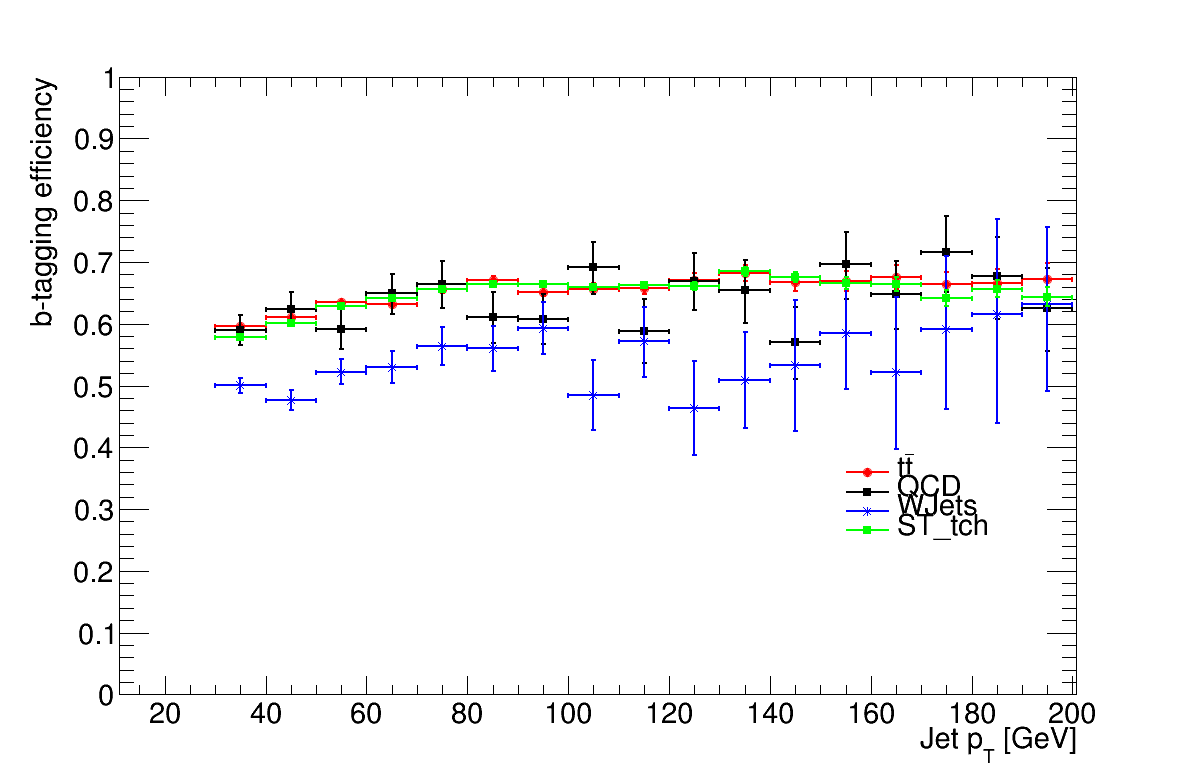
\includegraphics[scale=0.20]{genPlots/btagged/bTaggingEfficiency_pfCSVv2IVFM.png}
& \hspace{-0.5cm} 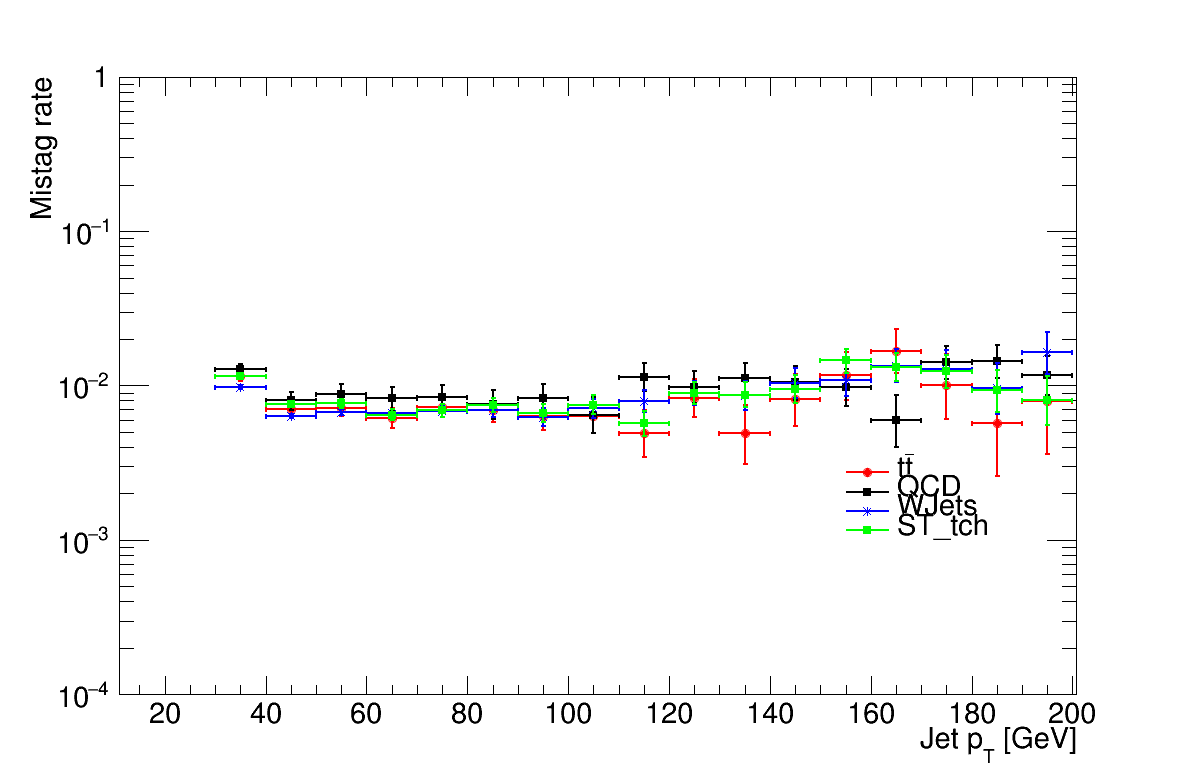
\includegraphics[scale=0.20]{genPlots/btagged/MistagRate_pfCSVv2IVFM.png}\\
   ($\mathbf{c}$)\qquad\qquad&($\mathbf{d}$)\qquad\qquad\qquad\\
\end{tabular}
\caption{(a): CSV for b, c and udsg jets (b): Log View of CSV for b, c and udsg jets}.\label{CSVforb_c_udsg_jets}
\end{figure}
%-------------------------------------------------------- 
\subsection{Higgs boson Reconstruction}
A Higgs boson is recontructed from $t\overline{t}$ using the kinematic reconstruction techniques. A $t\overline{t}$ event is recognized by the decay products of W boson and two b-tagged jets. We consider the semileptonic decay of $t\overline{t}$, where one of the W boson decays hadronically ($W\rightarrow q\acute{q}$) while the other decays leptonically ($W\rightarrow l + \not\mathrel{E}_{T}$). Leptonically decaying W boson is reconstructed using the lepton momentum and and the missing transvese energy ($\not\mathrel{E}_{T}$). We assume that the x and y components of missing transverse energy ($\not\mathrel{E}_{T}$) are entirely due to the escaping neutrino. By applying the W-mass constraint of 80.4 GeV, we extract the unkown longitudinal component ($p_{Z,v}$) of the missing transverse energy. This is done by using the quadratic equation:
\begin{equation}
m^{2}_{w} = {(E_{l}+\sqrt{\not\mathrel{E}^{2}_{T}+p^{2}_{Z,v}})}^{2}-{(\vec{p_{T,l}}+\vec{\not\mathrel{E}_{T}})}^{2}-{(p_{Z,l}+p_{Z,v})}^{2} 
\end{equation} 
This equation gives complex solution for about 30\% of the events. To get only the real solutions, x and y components of missing transverse energy ($\not\mathrel{E}_{T}$) are varied to get W boson transverse mass ($m_{T,w}$) of 80.4 GeV that makes the discriminant zero. The two non b-tagged jets that give mass near to 80.4 GeV are assign to hadronic top quark ($t_{had}$). The combination of lepton-neutrino-b-jet that gives mass near to 172.5 GeV reconstruct the leptonic top quark ($t_{lep}$). The remaining b-tagged jet combines to the selected pair of non b-tagged jets to reconstruct the hadronic top quark ($t_{had}$). The charge of muon separates top quark from anti-top. If muon charge is positive, the leptonic top quark is assign to top and hadronic top quark is anti top ($\overline{t}$) quark and vice versa. The top and anti top qurak combined to reconstruct a Higgs boson.
\begin{figure}[htp!]
\centering
%\begin{tabular}{cc}
\hspace{-0.5cm}

\includegraphics[scale=0.40]{diagrams/higgs_tottbar.png}
%  \end{tabular}
   \caption{Production and decay of a heavy Higgs boson}.\label{higgs_diagram}
    \end{figure}
%----------------------------------------------------------------------------------------------------
   
%--------------------------------------------------------
\section{Analysis Strategy}
%-----------------------------Number of vertices-----------------------
\begin{figure}[htp]
\centering
\begin{tabular}{cc}
\hspace{-0.5cm}
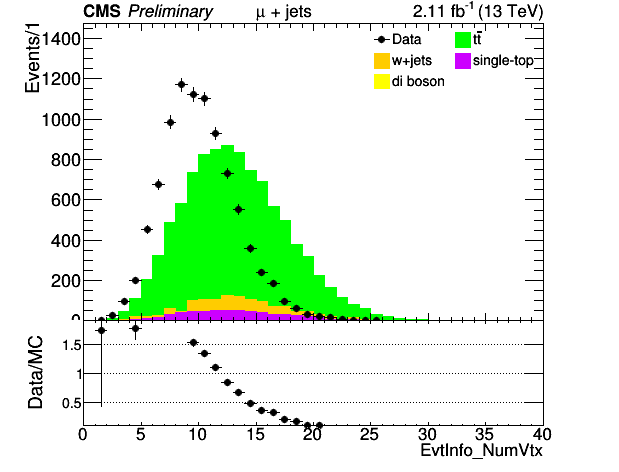
\includegraphics[scale=0.40]{results/EvtInfo_NumVtx.png}
& \hspace{-0.5cm} 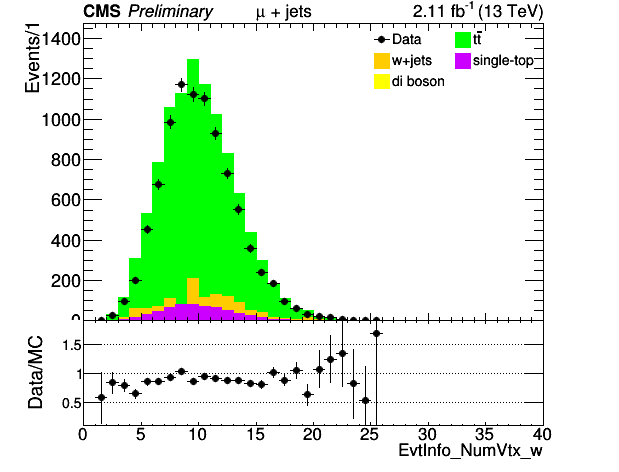
\includegraphics[scale=0.40]{results/EvtInfo_NumVtx_w.png}\\
   ($\mathbf{a}$)\qquad\qquad&($\mathbf{b}$)\qquad\qquad\qquad\\
\hspace{-0.5cm}
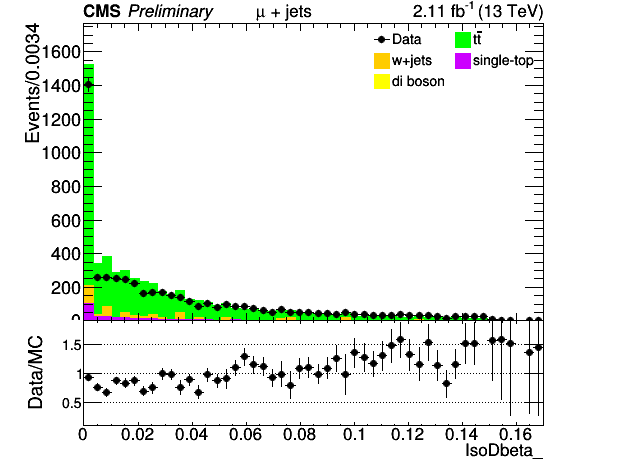
\includegraphics[scale=0.40]{results/IsoDbeta_.png}
& \hspace{-0.5cm} 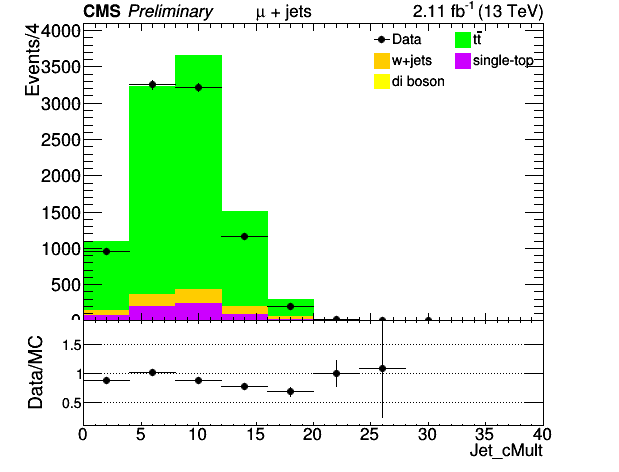
\includegraphics[scale=0.40]{results/Jet_cMult.png}\\
   ($\mathbf{c}$)\qquad\qquad&($\mathbf{d}$)\qquad\qquad\qquad\\
\end{tabular}
\caption{(a): No. of vertices with no weight (b): weighted no. of vertices (c) Isolation variable with $\delta\beta$ correction (d) Jets charge multiplicity.}\label{no_vertex}
\end{figure}

%-----------------------------jets-------------------------------------
\begin{figure}[htp]
\centering
\begin{tabular}{cc}
\hspace{-0.5cm}
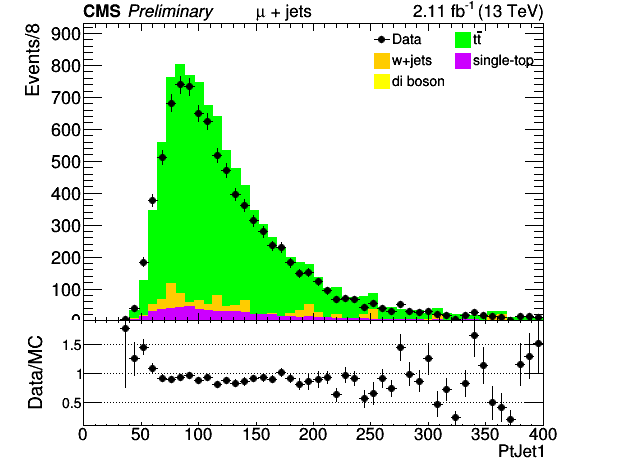
\includegraphics[scale=0.40]{results/PtJet1.png}
& \hspace{-0.5cm} 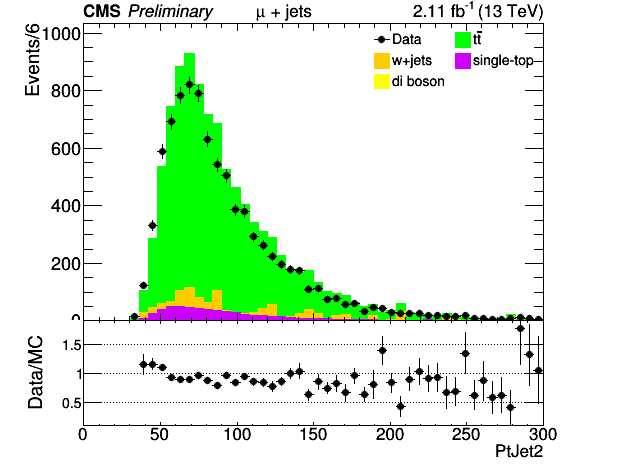
\includegraphics[scale=0.40]{results/PtJet2.png}\\
   ($\mathbf{a}$)\qquad\qquad&($\mathbf{b}$)\qquad\qquad\qquad\\
\hspace{-0.5cm}
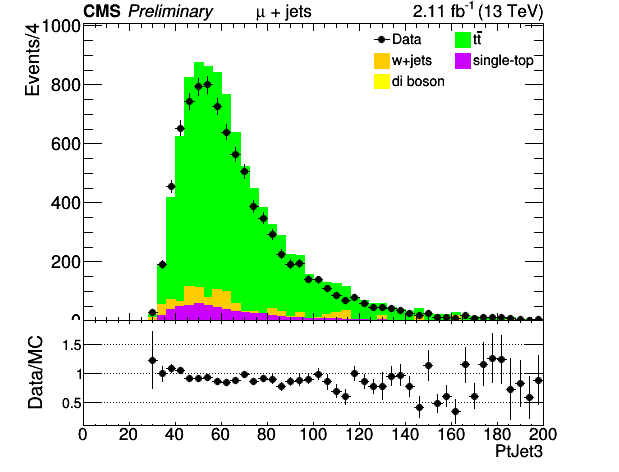
\includegraphics[scale=0.40]{results/PtJet3.png}
& \hspace{-0.5cm} 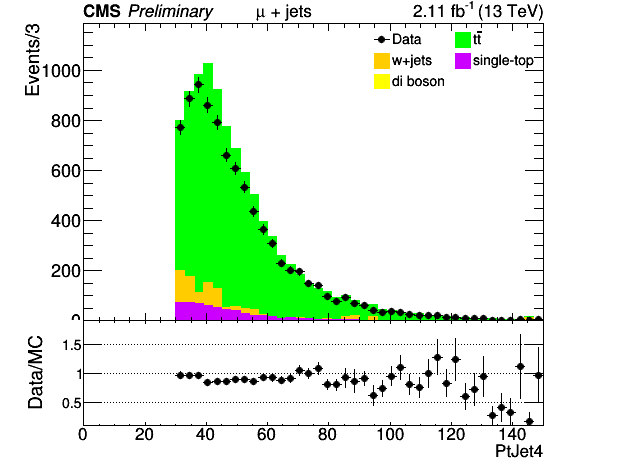
\includegraphics[scale=0.40]{results/PtJet4.png}\\
   ($\mathbf{c}$)\qquad\qquad&($\mathbf{d}$)\qquad\qquad\qquad\\
\end{tabular}
\caption{$p_{T}$ of (a): 1$^{st}$ jet (b): 2$^{nd}$ jet (c): 3$^{rd}$ jet (4): 4$^{th}$ jet.}\label{Pts_jets}
\end{figure}
%--------------------
\begin{figure}[htp]
\centering
\begin{tabular}{cc}
\hspace{-0.5cm}
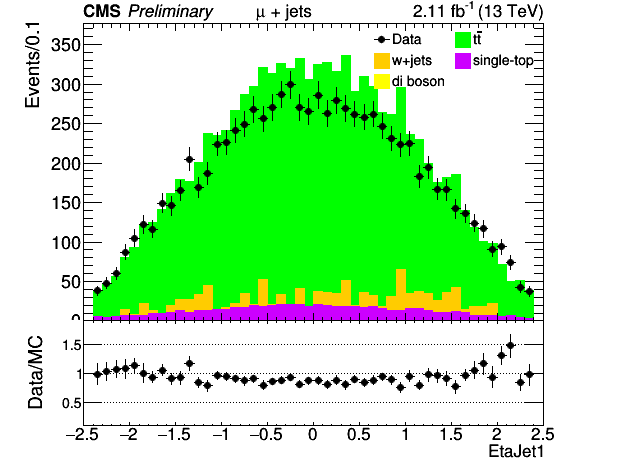
\includegraphics[scale=0.40]{results/EtaJet1.png}
& \hspace{-0.5cm} 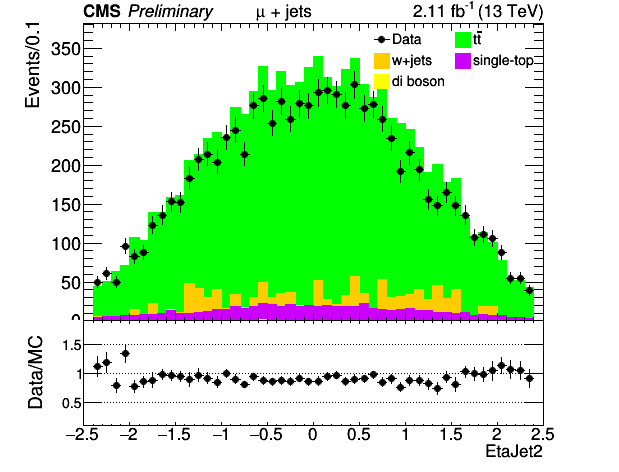
\includegraphics[scale=0.40]{results/EtaJet2.png}\\
   ($\mathbf{a}$)\qquad\qquad&($\mathbf{b}$)\qquad\qquad\qquad\\
\hspace{-0.5cm}
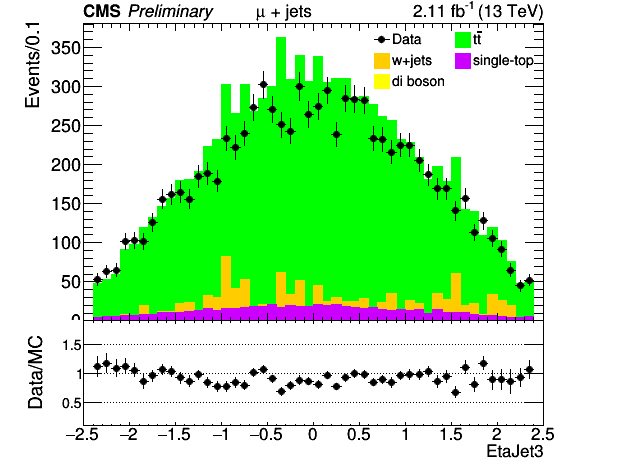
\includegraphics[scale=0.40]{results/EtaJet3.png}
& \hspace{-0.5cm} 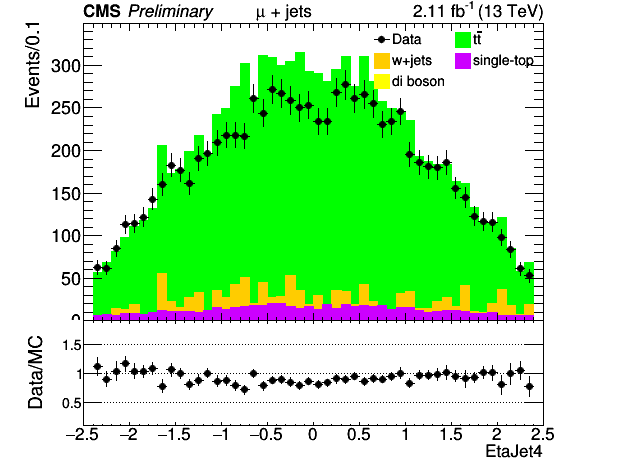
\includegraphics[scale=0.40]{results/EtaJet4.png}\\
   ($\mathbf{c}$)\qquad\qquad&($\mathbf{d}$)\qquad\qquad\qquad\\
\end{tabular}
\caption{$\eta$ of (a): 1$^{st}$ jet (b): 2$^{nd}$ jet (c): 3$^{rd}$ jet (d): 4$^{th}$ jet.}\label{etas_jets}
\end{figure}
%------------------------------------bjets Pts and etas------------------
\begin{figure}[htp]
\centering
\begin{tabular}{cc}
\hspace{-0.5cm}
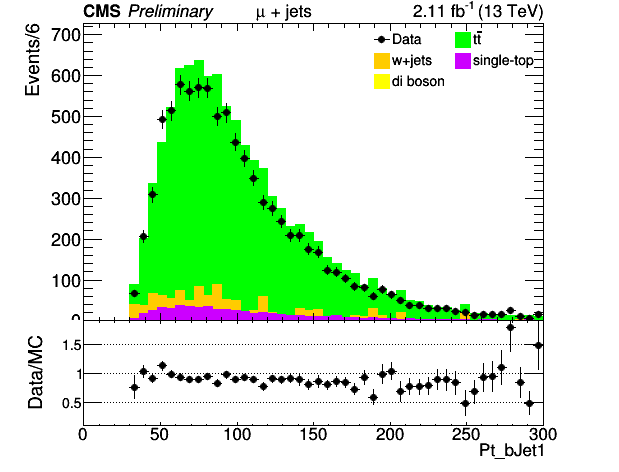
\includegraphics[scale=0.40]{results/Pt_bJet1.png}
& \hspace{-0.5cm} 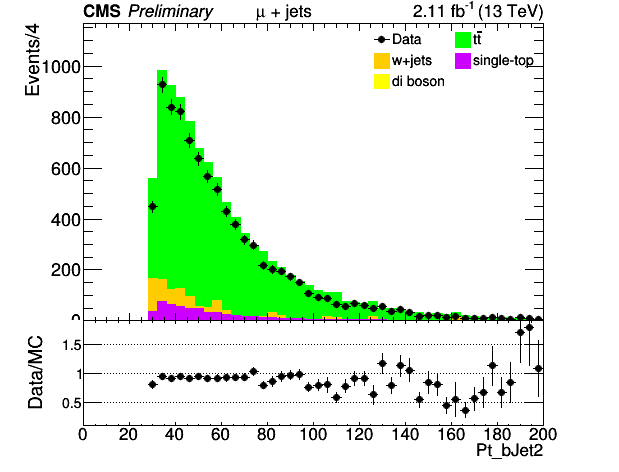
\includegraphics[scale=0.40]{results/Pt_bJet2.png}\\
   ($\mathbf{a}$)\qquad\qquad&($\mathbf{b}$)\qquad\qquad\qquad\\
\hspace{-0.5cm}
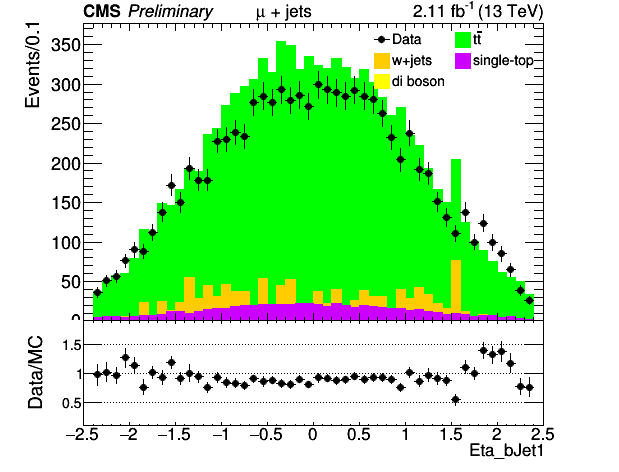
\includegraphics[scale=0.40]{results/Eta_bJet1.png}
& \hspace{-0.5cm} 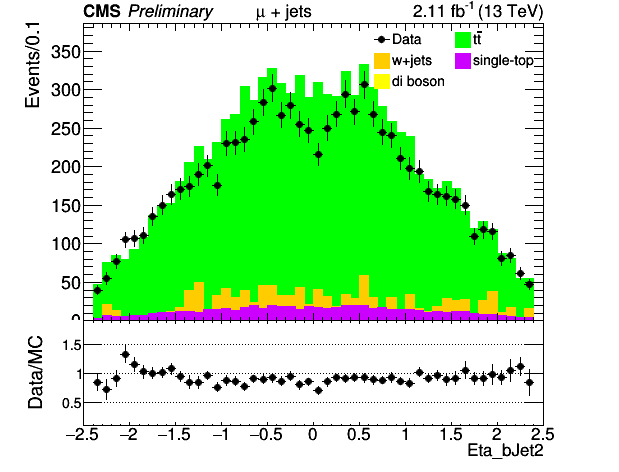
\includegraphics[scale=0.40]{results/Eta_bJet2.png}\\
   ($\mathbf{c}$)\qquad\qquad&($\mathbf{d}$)\qquad\qquad\qquad\\
\end{tabular}
\caption{$p_{T}$ of (a): 1$^{st}$ bjet (b): 2$^{nd}$ bjet. $\eta$ of (c): 1$^{st}$ bjet (d): 2$^{nd}$ bjet.}\label{Pts_etas_bjets}
\end{figure}
%------------------------------------ljets pts and etas-------------------
\begin{figure}[htp]
\centering
\begin{tabular}{cc}
\hspace{-0.5cm}
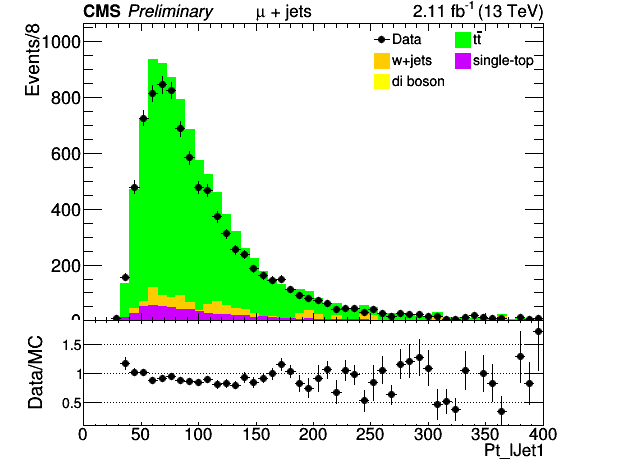
\includegraphics[scale=0.40]{results/Pt_lJet1.png}
& \hspace{-0.5cm} 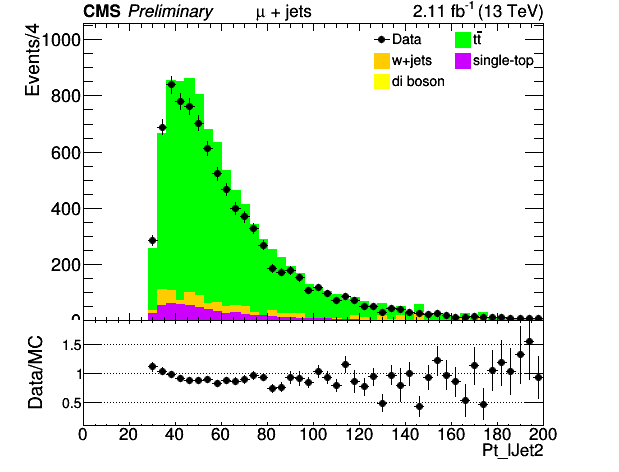
\includegraphics[scale=0.40]{results/Pt_lJet2.png}\\
   ($\mathbf{a}$)\qquad\qquad&($\mathbf{b}$)\qquad\qquad\qquad\\
\hspace{-0.5cm}
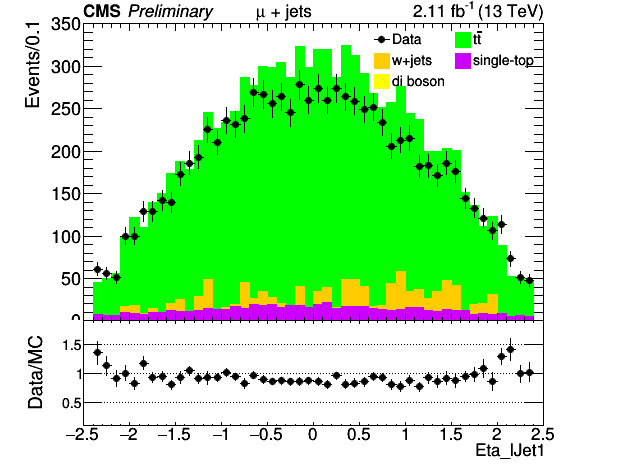
\includegraphics[scale=0.40]{results/Eta_lJet1.png}
& \hspace{-0.5cm} 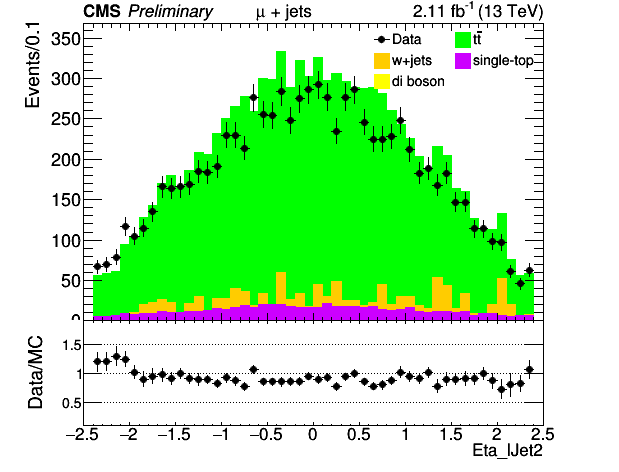
\includegraphics[scale=0.40]{results/Eta_lJet2.png}\\
   ($\mathbf{c}$)\qquad\qquad&($\mathbf{d}$)\qquad\qquad\qquad\\
\end{tabular}
\caption{$p_{T}$ of (a): 1$^{st}$ non-bjet (b): 2$^{nd}$ non-bjet. $\eta$ of (c): 1$^{st}$ non-bjet (d): 2$^{nd}$ non-bjet.}\label{Pts_etas_ljets}
\end{figure}
%------------------------------------Muon and MET--------------------------
\begin{figure}[htp]
\centering
\begin{tabular}{cc}
\hspace{-0.5cm}
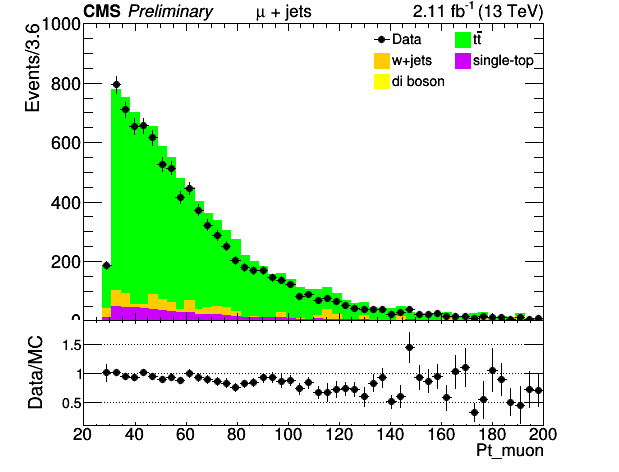
\includegraphics[scale=0.40]{results/Pt_muon.png}
& \hspace{-0.5cm} 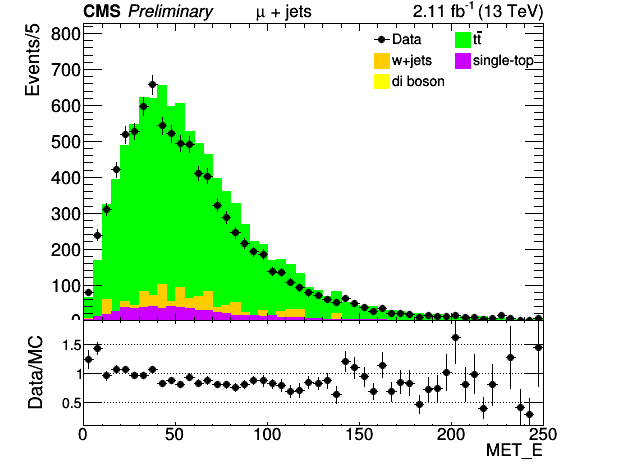
\includegraphics[scale=0.40]{results/MET_E.png}\\
   ($\mathbf{a}$)\qquad\qquad&($\mathbf{b}$)\qquad\qquad\qquad\\
\hspace{-0.5cm}
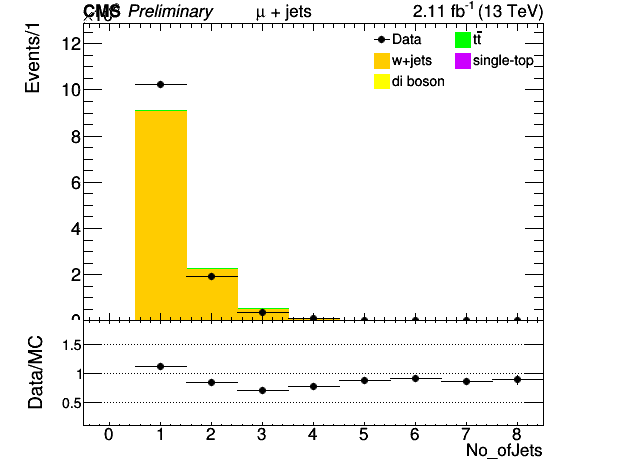
\includegraphics[scale=0.40]{results/No_ofJets.png}
& \hspace{-0.5cm} 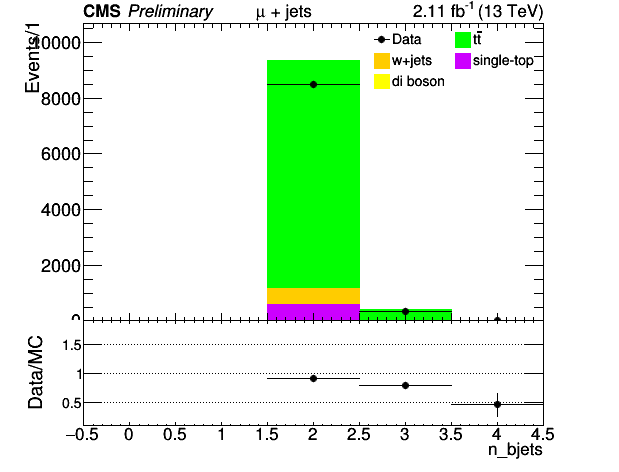
\includegraphics[scale=0.40]{results/n_bJets.png}\\
   ($\mathbf{c}$)\qquad\qquad&($\mathbf{d}$)\qquad\qquad\qquad\\
\end{tabular}
\caption{(a): $p_{T}$ of muon (b): missing transverse energy (c): number of jets (d): number of b-jets.}\label{muon}
\end{figure}
%-------------------------------------W bosons ------------------------------
\begin{figure}[htp]
\centering
\begin{tabular}{cc}
\hspace{-0.5cm}
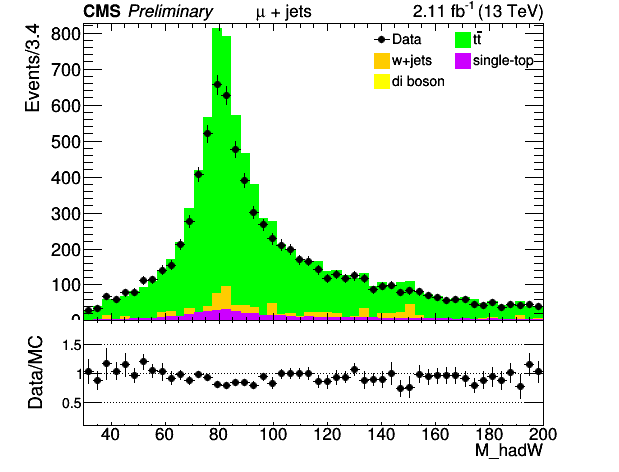
\includegraphics[scale=0.40]{results/M_hadW.png}
& \hspace{-0.5cm} 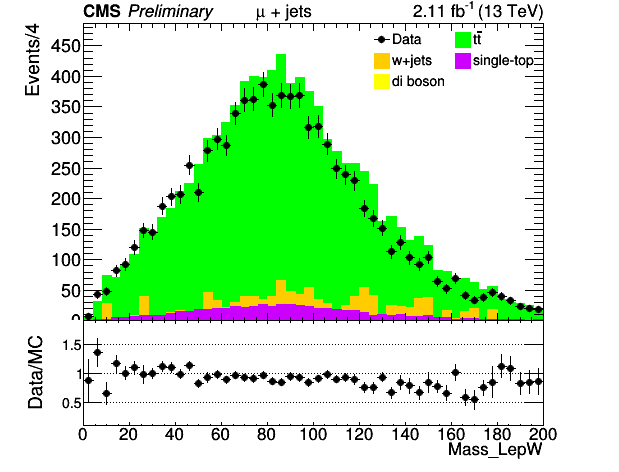
\includegraphics[scale=0.40]{results/mass_LepW.png}\\
   ($\mathbf{a}$)\qquad\qquad&($\mathbf{b}$)\qquad\qquad\qquad\\
\hspace{-0.5cm}
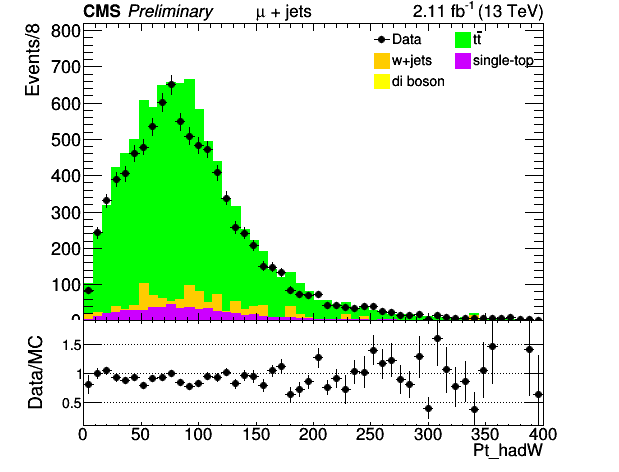
\includegraphics[scale=0.40]{results/Pt_hadW.png}
& \hspace{-0.5cm} 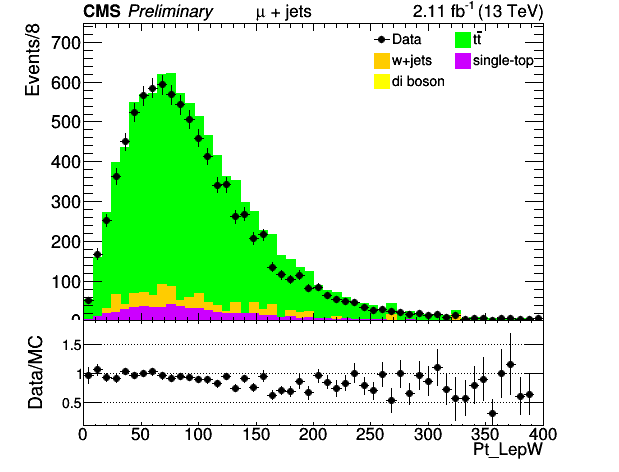
\includegraphics[scale=0.40]{results/Pt_LepW.png}\\
   ($\mathbf{c}$)\qquad\qquad&($\mathbf{d}$)\qquad\qquad\qquad\\
\end{tabular}
\caption{(a): mass of hadronic W boson (b): mass of leptonic W boson (c): $p_{T}$ of hadronic W boson (d): $p_{T}$ of leptonic W boson.}\label{W_boson}
\end{figure}
%------------------------------------top quarks------------------------------
\begin{figure}[htp]
\centering
\begin{tabular}{cc}
\hspace{-0.5cm}
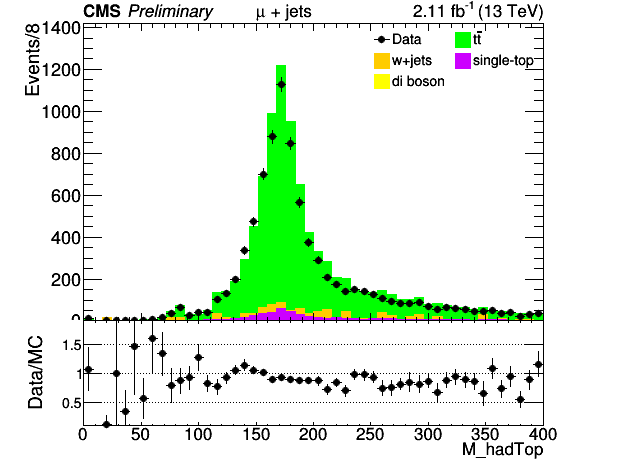
\includegraphics[scale=0.40]{results/M_hadTop.png}
& \hspace{-0.5cm} 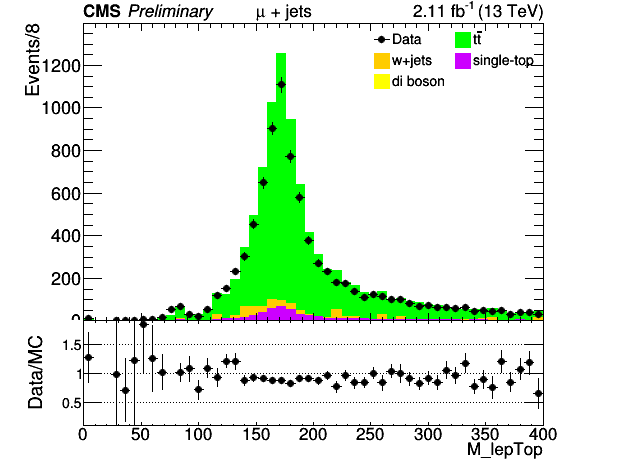
\includegraphics[scale=0.40]{results/M_lepTop.png}\\
   ($\mathbf{a}$)\qquad\qquad&($\mathbf{b}$)\qquad\qquad\qquad\\
\hspace{-0.5cm}
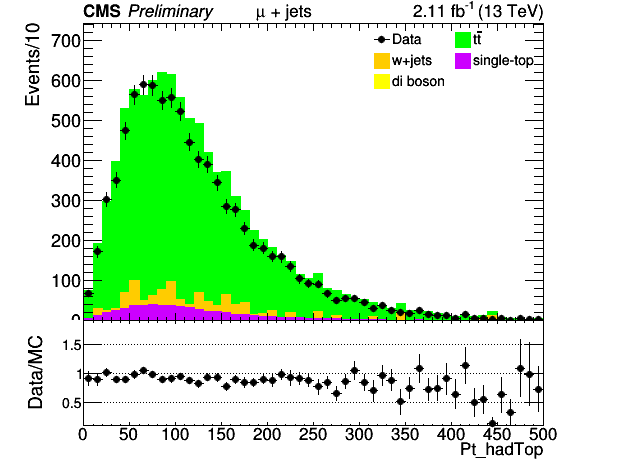
\includegraphics[scale=0.40]{results/Pt_hadTop.png}
& \hspace{-0.5cm} 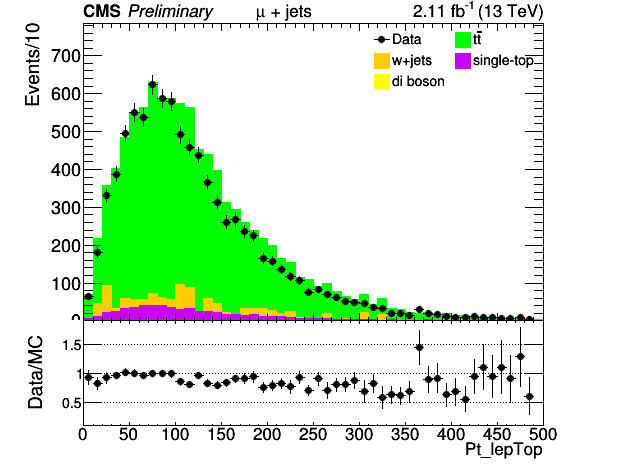
\includegraphics[scale=0.40]{results/Pt_lepTop.png}\\
   ($\mathbf{c}$)\qquad\qquad&($\mathbf{d}$)\qquad\qquad\qquad\\
\end{tabular}
\caption{(a): mass of $\overline{t}$ (b): mass of top (c): $p_{T}$ of $\overline{t}$ (d): $p_{T}$ of top.}\label{W_boson}
\end{figure}
%------------------------------------ttbar ------------------------------------
\begin{figure}[!htp]
\centering
\begin{tabular}{cc}
\hspace{-0.5cm}
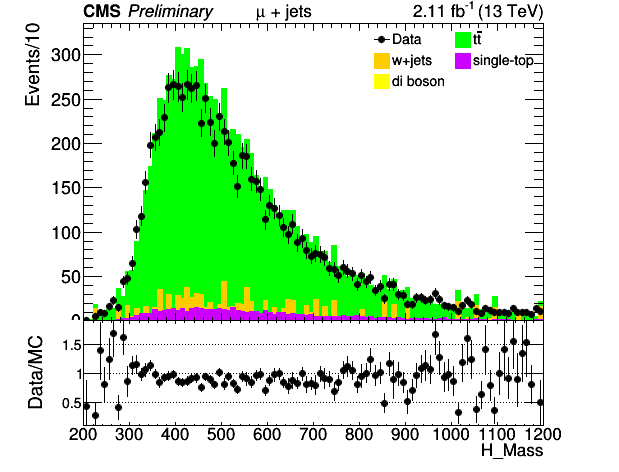
\includegraphics[scale=0.40]{results/Mass_H.png}
& \hspace{-0.5cm} 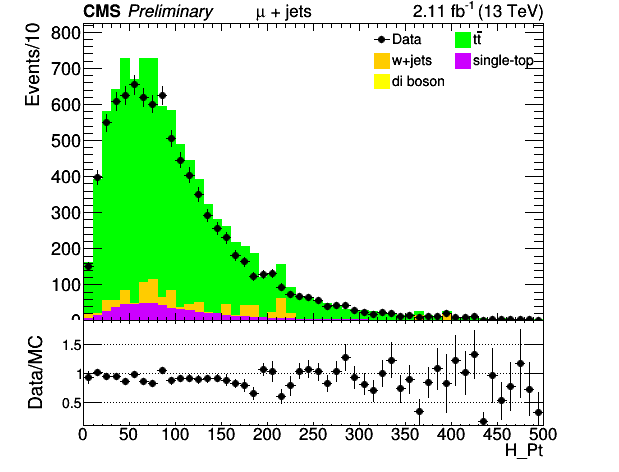
\includegraphics[scale=0.40]{results/Pt_H.png}\\
   ($\mathbf{a}$)\qquad\qquad&($\mathbf{b}$)\qquad\qquad\qquad\\
%\hspace{-0.5cm}
%\includegraphics[scale=0.40]{results/events_eachCut.png}
%& \hspace{-0.5cm} \includegraphics[scale=0.40]{results/Pt_lepTop.png}\\
 %  ($\mathbf{c}$)\qquad\qquad&($\mathbf{d}$)\qquad\qquad\qquad\\
\end{tabular}
\caption{(a): mass of $\overline{t}$ (b): mass of top (c): $p_{T}$ of $\overline{t}$ (d): $p_{T}$ of top.}\label{W_boson}
\end{figure}

\clearpage
\section{Discussion and Conclusions}

\section{Acknowledgements}

\section{Appendix}
%\begin{equation}
%\frac{1}{\sigma}\frac{d\sigma}{d\cos\theta_i}=\frac{1+\alpha_i\cos\theta_i}{2}
%\end{equation}
%\begin{equation}
%\frac{d^2\sigma}{d\cos\theta_1d\cos\theta_2}=\frac{\sigma(1-C\cos\theta_1d\cos\theta_2)}{4}
%\end{equation}
%where $\theta_i$ is the angle between the direction of the decay leptons (or jets from W's) and the spin-quantization axis in the parent t and $\bar{t}$ rest frames and  $C=A\alpha_1\alpha_2$.
\clearpage
 \begin{thebibliography}{99}
% \bibitem{ref:newphysics1} D. London and J.L. Rosner 1986 {\it Phys. Rev. D} {\bf 34} 1530
\bibitem{HiggsCMS}CMS Collaboration, ``Observation of a new boson at a mass of 125 GeV with the CMS experiment at the LHC", \textit{Phys. Lett.} \textbf{B 716} (2012) 30, \href{http://www.sciencedirect.com/science/article/pii/S0370269312008581}{\texttt{doi:10.1016/j.physletb.2012.08.021}}, \href{http://arxiv.org/abs/1207.7235v2}{\texttt{arXiv:1207.7235v2}}.
\bibitem{HiggsATLAS}ATLAS Collaboration, ``Observation of a New Particle in the Search for the Standard Model Higgs Boson with the ATLAS Detector at the LHC", \textit{Phys. Lett}. \textbf{B 716} (2012) 1-29, \href{http://www.sciencedirect.com/science/article/pii/S037026931200857X}{\texttt{doi:10.1016/j.physletb.2012.08.020}}, \href{http://arxiv.org/abs/1207.7214}{\texttt{arXiv:1207.7214v2}}.
\bibitem{5584}W. Bernreuther et al., ``Production of Heavy Higgs bosons and decay into top quarks at the LHC", \href{http://arxiv.org/abs/1511.05584}{\texttt{arXiv:1511.05584v1}}.
\bibitem{2HDM}G. C. Branco et al., ``Theory and phenomenology of two-Higgs-doublet models", \textit{Phys. Report}, \href{http://www.sciencedirect.com/science/article/pii/S0370157312000695}{\texttt{doi:10.1016/j.physrep.2012.02.002}}, \href{http://arxiv.org/abs/1106.0034}{\texttt{arXiv:1106.0034v3}}.
\bibitem{SignHiggs}W. Bernreuther et al., ``Signature of Higgs bosons in the Top Quark Decay Channel at Hadron Colliders", \textit{Phys. Rev.} \textbf{D 58} (1998) 114031, \href{http://journals.aps.org/prd/abstract/10.1103/PhysRevD.58.114031}{\texttt{doi:10.1103/PhysRevD.58.114031}}, \href{http://arxiv.org/pdf/hep-ph/9709284.pdf}{\texttt{arXiv:hep-ph/9709284}}.
\bibitem{magnet}CMS Collaboration, ``The Magnet Project Technical Design Report", CERN-LHCC-97-010, \href{http://cdsweb.cern.ch/record/331056}{\texttt{http://cdsweb.cern.ch/record/331056}}.
\bibitem{rpc}M. Tytgat et al., ``The Upgrade of the CMS RPC System during the First LHC Long Shutdown", XI workshop on Resistive Plate Chambers and Related Detectors (RPC2012), \href{http://iopscience.iop.org/article/10.1088/1748-0221/8/02/T02002/meta}{\texttt{doi:10.1088/1748-0221/8/02/T02002}}, \href{http://arxiv.org/abs/1209.1979}{\texttt{arXiv:1209.1979}}
\bibitem{cmsdetector}CMS Collaboration, ``The CMS experiment at the CERN LHC", \textit{JINST} \textbf{3} (2008) S08004, \href{http://iopscience.iop.org/article/10.1088/1748-0221/3/08/S08004/meta;jsessionid=169D4C0CEE0D0ECD3FAC1D1C8C8B2CB2.c1.iopscience.cld.iop.org}{\texttt{doi:10.1088/1748-0221/3/08/S08004}}.
\bibitem{madgraph}J. Alwall et al., ``The automated computation of tree-level and next-to-leading order differential cross sections, and their matching to parton shower simulations", \textit{JHEP} \textbf{07} (2014)079, \href{http://link.springer.com/article/10.1007\%2FJHEP07\%282014\%29079}{\texttt{doi:10.1007/JHEP07(2014)079}}, \href{http://arxiv.org/abs/1405.0301}{\texttt{arXiv:1405.0301v2}}.
\bibitem{signal1}R. Frederix \& F. Maltoni, ``Top pair invariant mass distribution: a window on new physics", \textit{JHEP} 0901:047,2009, \href{http://iopscience.iop.org/article/10.1088/1126-6708/2009/01/047/meta;jsessionid=B54EB5B24AAF6EF0497D870A84C91AF3.c2.iopscience.cld.iop.org}{\texttt{doi:10.1088/1126-6708/2009/01/047}}, \href{http://arxiv.org/abs/0712.2355}{\texttt{arXiv:0712.2355}}.  
\bibitem{signal2}K. J. F. Gaemers, F. Hoogeveen, ``Higgs production and decay into heavy flavours with the gluon fusion mechanism", \textit{Phys. Lett.} \textbf{B}, \href{http://www.sciencedirect.com/science/article/pii/0370269384917118}{\texttt{doi:10.1016/0370-2693(84)91711-8}}.
\bibitem{signal3}D. Dicus, A. Stange, S. Willenbrock, ``Higgs Decay to Top Quarks at Hadron Colliders", \textit{Phys. Lett.} \textbf{B333} (1994) 126-131, \href{http://www.sciencedirect.com/science/article/pii/0370269394910170}{\texttt{doi:10.1016/0370-2693(94)91017-0}}, \href{http://arxiv.org/abs/hep-ph/9404359}{\texttt{arXiv:hep-ph/9404359}}
\bibitem{signal4}\href{https://github.com/blinkseb/HTTMadgraphDocumentation/blob/master/README.md}{\texttt{github.com/blinkseb/HTTMadgraphDocumentation/blob/master/README.md}}.
\bibitem{sabisteinPAS}CMS Collaboration, ``Search for massive scalar particles decaying to $t\overline{t}$ pairs in the semileptonic final state", \href{http://cms.cern.ch/iCMS/analysisadmin/cadilines?line=B2G-14-007}{\texttt{B2G-14-007}}.
\bibitem{fastsim}\href{https://twiki.cern.ch/twiki/bin/view/CMSPublic/SWGuideFastSimulationExamples#Run2\_Spring15\_recipe}{\texttt{SWGuideFastSimulationExamples-Run2-Spring15-recipe}}.
\bibitem{muonid}https://twiki.cern.ch/twiki/bin/view/CMSPublic/SWGuideMuonId.
\bibitem{Akt}M. Cacciari et al., ``The anti-$k_{t}$ jet clustering algorithm", \textit{JHEP} \textbf{04} (2008)063, \href{http://iopscience.iop.org/article/10.1088/1126-6708/2008/04/063/meta}{\texttt{doi:10.1088/1126-6708/2008/04/063}}, \href{http://arxiv.org/abs/0802.1189}{\texttt{arXiv:0802.1189}}
\bibitem{jet-reco}M. Schoder, ``Performance of jets at CMS", Journal of Physics: Conference Series \textbf{587} (2015) 012004, \href{http://iopscience.iop.org/article/10.1088/1742-6596/587/1/012004/meta}{\texttt{doi:10.1088/1742-6596/587/1/012004}}.
\bibitem{bjet}CMS Collaboration, ``Identification of b-quark jets with the CMS experiment", \textit{JINST} \textbf{8} (2013) P04013, \href{http://iopscience.iop.org/article/10.1088/1748-0221/8/04/P04013/meta}{\texttt{doi:10.1088/1748-0221/8/04/P04013}}, \href{http://arxiv.org/abs/1211.4462}{\texttt{arXiv:1211.4462}}.
%%\addcontentsline{toc}{chapter}{Bibliography}

%%\bibliographystyle{unsrt}

\bibliographystyle{acm}

%%\bibliography{XBib}
 \end{thebibliography}
 
 
 

 \end{document}
% 
